%!TEX root = ../thesis.tex

\section{Результати дослідження}
\label{chap:research_results} 

В результаті проробленої роботи було визначено, що детерміністична та стохастична функції вийшли різними, при цьому значення обох середніх похибок у відповідних функціях вийшли однаковими. Таким чином, отримали, що обидві функції досить добре підходять для нашого розподілу.

\subsection{Опис алгоритмів побудови вирішуючих функцій}

Алгоритми побудови вирішуючих функцій схожі між собою і безпосередньо відрізняються лише останнім кроком.

Наведемо алгоритми для обчислення детерміністичної та стохастичної функцій:

\begin{algorithm}
    Побудова детерміністичної вирішуючої функції.
    \begin{itemize}
    \large
        \item Обчислюємо $P(C)$ за формулою:$\forall C: P(C) = \sum_{(M,k):E_k(M)=C} P(M,k)$.
        \item Обчислюємо $P(C)$ за формулою: $\forall (M,C): P(M,C) = \sum_{k:E_k(M)=C} P(M,k)$.
        \item Обчислюємо $P(M|C)$ за формулою $\frac{P(M,C)}{P(C)}$.
        \item З отриманих значень треба обрати максимальні та присвоїти значення $1$ до комірок матриці, де містилось дане максимальне значення. 
    \end{itemize}
\end{algorithm}

\begin{algorithm}
    Побудова стохастичної вирішуючої функції.
    \begin{itemize}
    \large
        \item Обчислюємо $P(C)$ за формулою:$\forall C: P(C) = \sum_{(M,k):E_k(M)=C} P(M,k)$.
        \item Обчислюємо $P(C)$ за формулою: $\forall (M,C): P(M,C) = \sum_{k:E_k(M)=C} P(M,k)$.
        \item Обчислюємо $P(M|C)$ за формулою $\frac{P(M,C)}{P(C)}$.
        \item З отриманих значень треба обрати максимальні та присвоїти значення $\frac{1}{s}$ до тих комірок матриці, де дане максимальне значення повторюється у рядку $s$ разів. 
    \end{itemize}
\end{algorithm}

\newpage
\subsection{Таблиця ймовірностей \textit{P(M|C)}}
\vspace{-1cm}
\begin{figure}[!h]
    \centering
    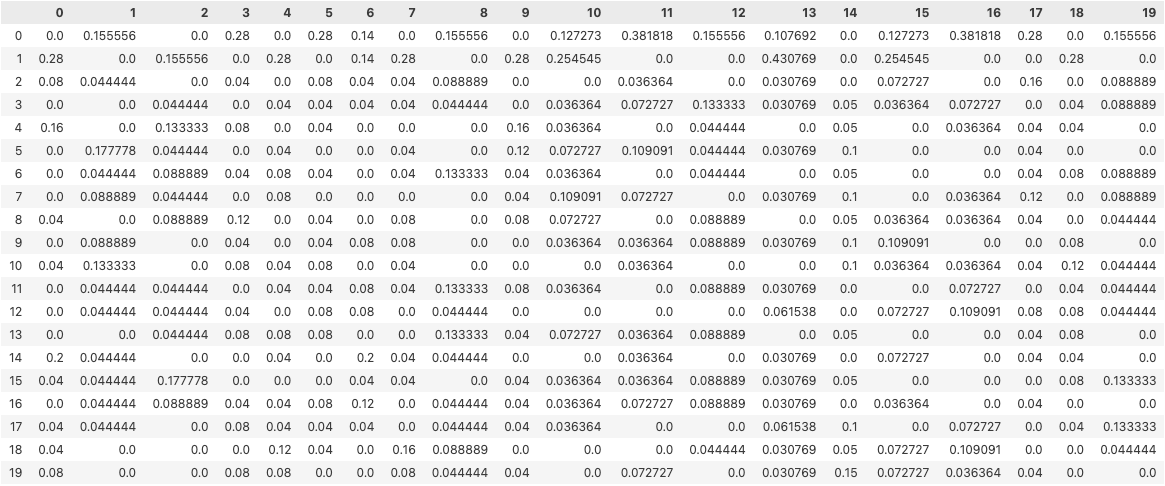
\includegraphics[scale = 0.42]{IMAGES/probabilityTable.png}
    \caption{\large Таблиця умовних ймовірностей для обчислення вирішуючих функцій.}
    \label{fig1}
\end{figure}
\vspace{-0.5cm}
\subsection{Детерміністична та стохастична матриці}
\vspace{-1cm}
\begin{figure}[!h]
    \centering
    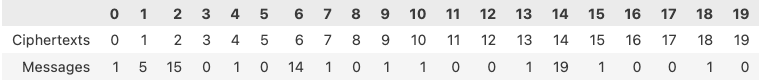
\includegraphics[scale = 0.5]{IMAGES/deterministicMatrix.png}
    \caption{\large Детерміністична вирішуюча ф-я у вигляді відображень (ШТ$\rightarrow$ВТ).}
    \label{fig2}
\end{figure}

\vspace{-1cm}
\begin{figure}[!h]
    \centering
    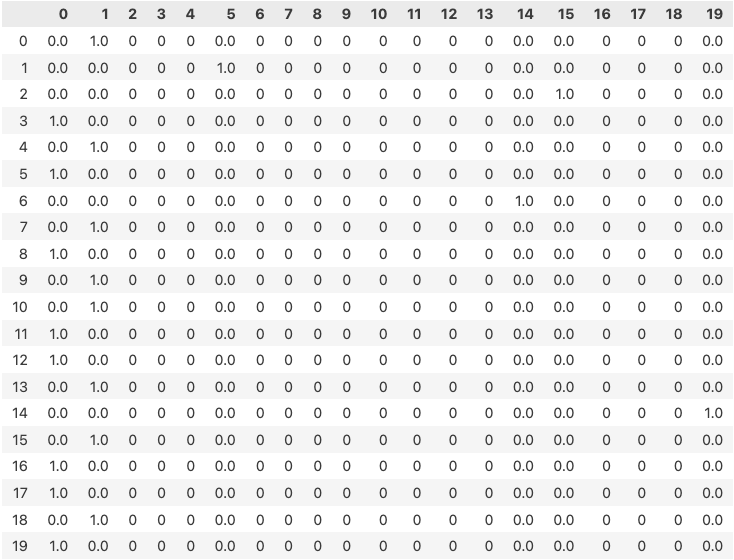
\includegraphics[scale = 0.4]{IMAGES/stohasticMatrix.png}
    \caption{\large Стохастична вирішуюча функція.}
    \label{fig3}
\end{figure}

Також було отримано наступні середні значення втрат:
\begin{itemize}
    \item Для детерміністичної функції: $0.737$
    \item Для стохастичної функції: $0.737$.
\end{itemize}